\section{Comparaion de protéines}

\subsection{Structure}
\begin{frame}{Recherche du plus grand sous-graphe isomorphe}
    \scriptsize
    \begin{figure}[!htb]
    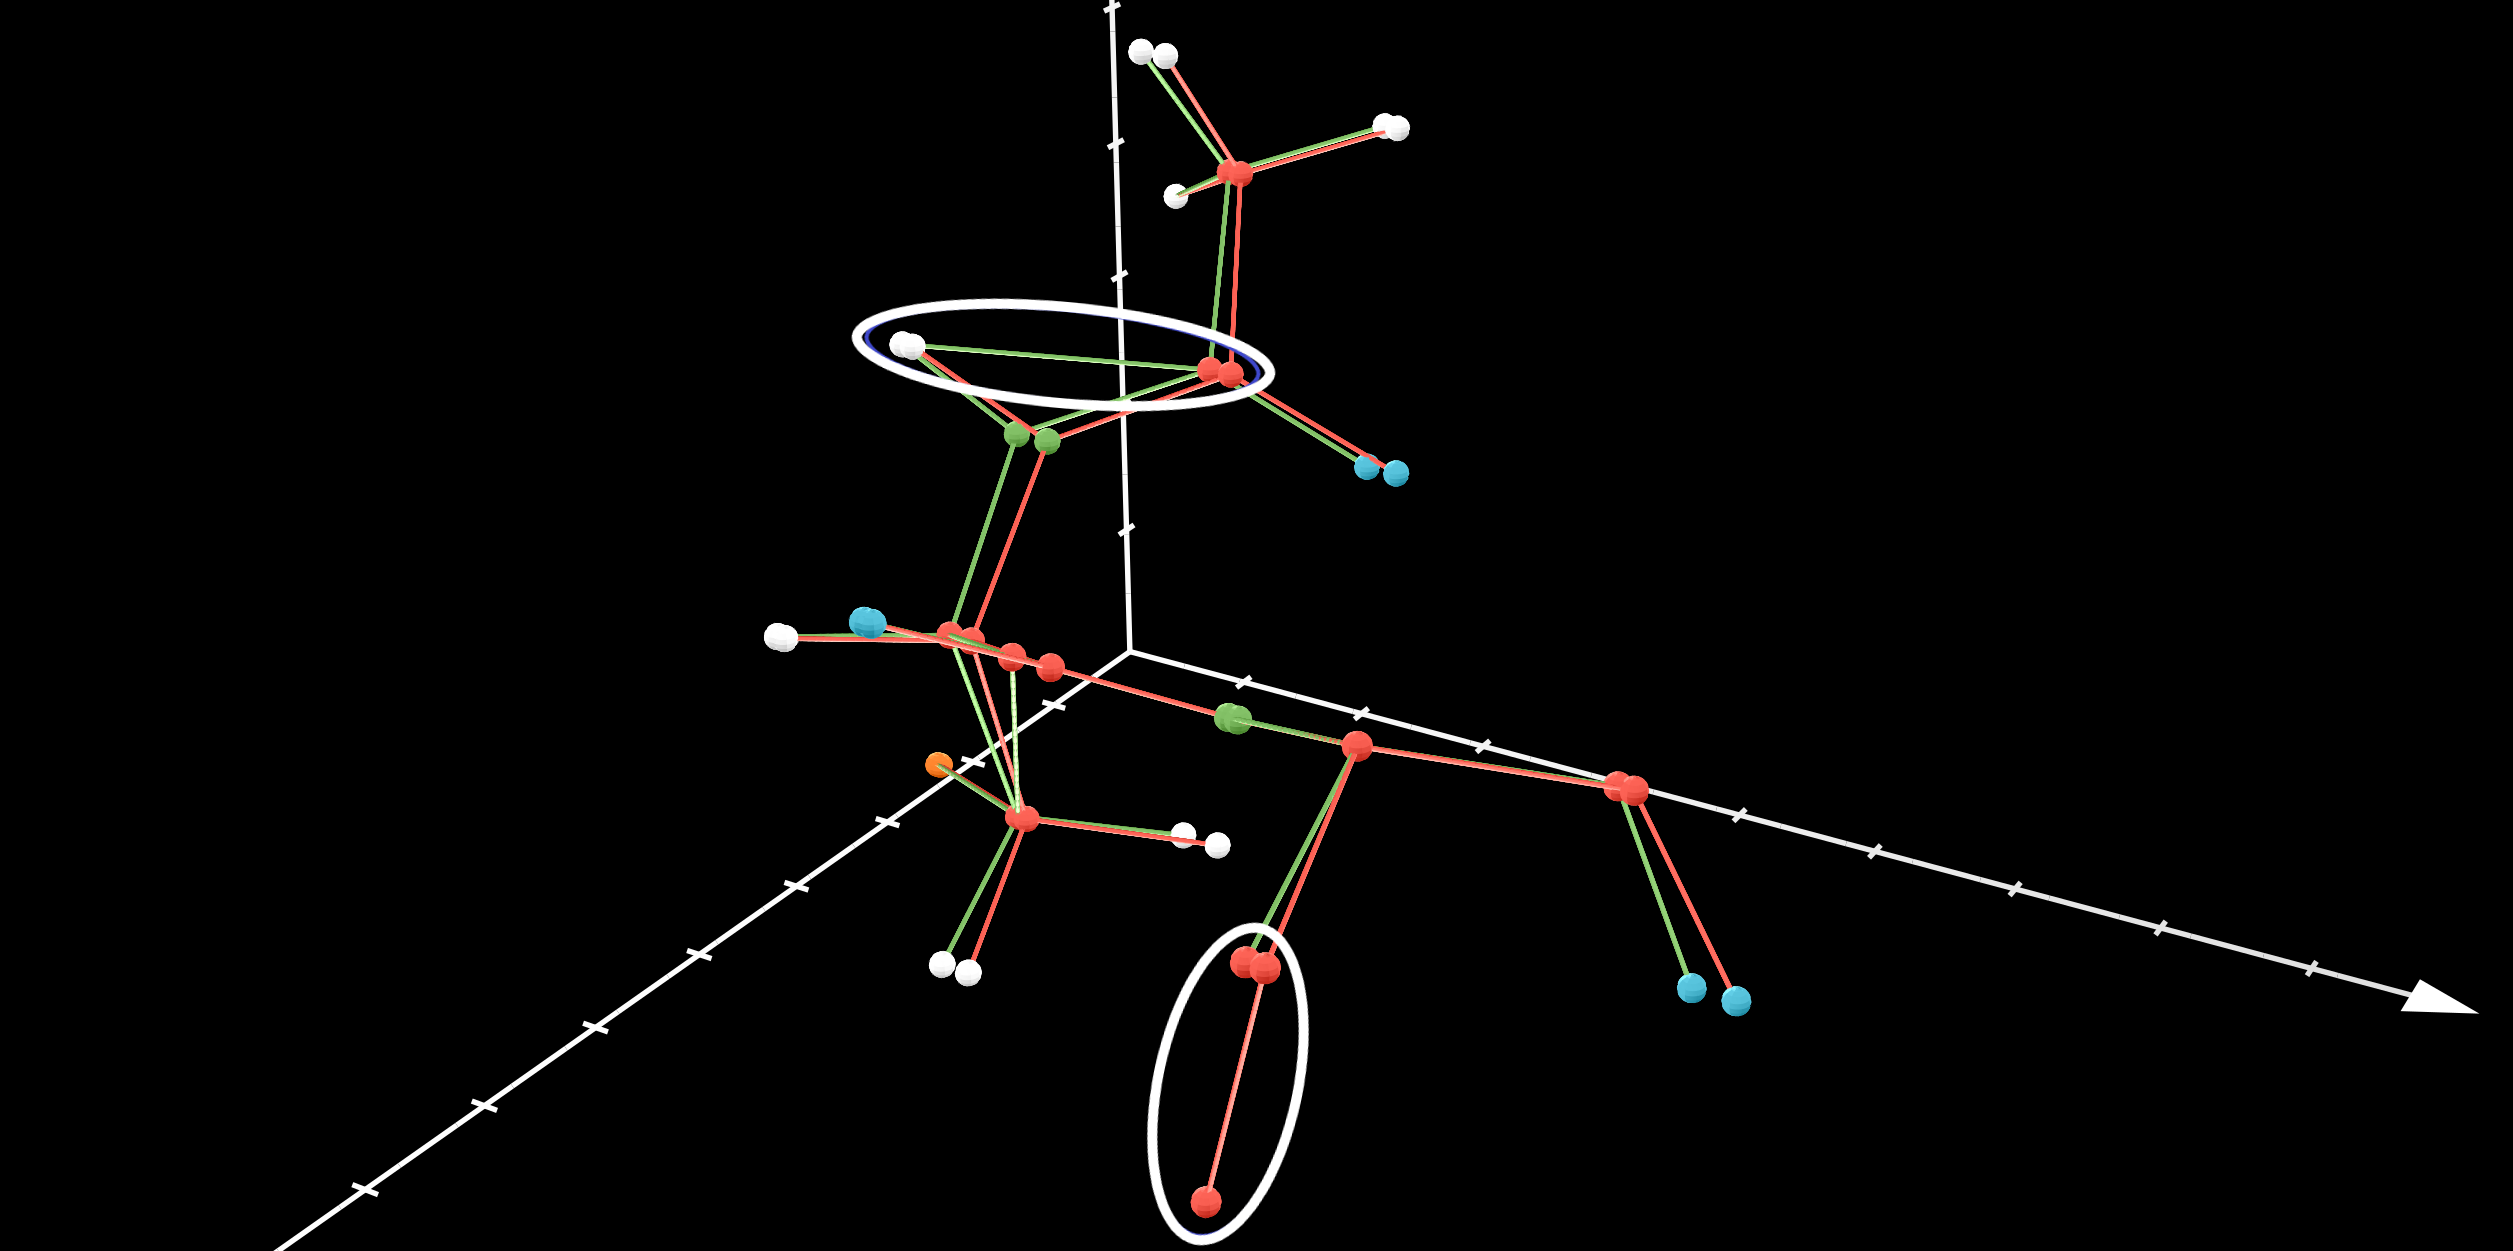
\includegraphics[width = 8.6cm]{comp_sub_largeview}
    \end{figure}
    \begin{multicols}{2}
        \begin{figure}[!htb]
            \centering
            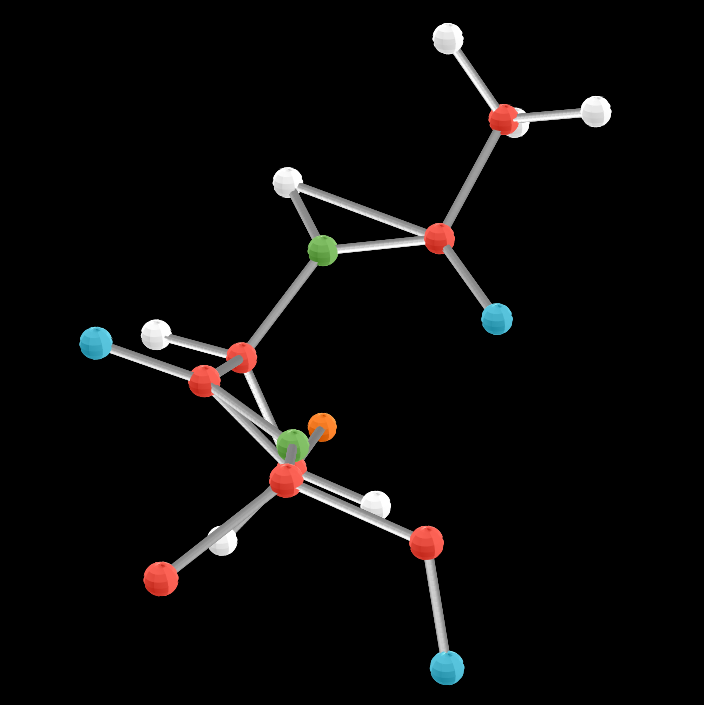
\includegraphics[width = 3cm]{sub1_lim22}
            \caption{\label{fig: sub1}Protéine de 21 atomes (en vert)}
        \end{figure}
        \begin{figure}[!htb]
            \centering
            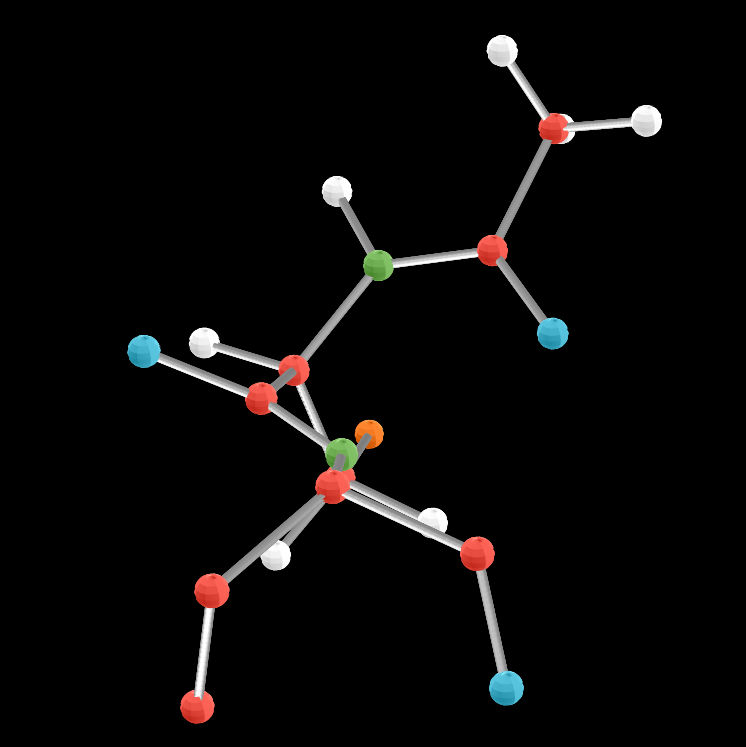
\includegraphics[width = 3cm]{sub2_lim22}
            \caption{\label{fig: sub2}Protéine de 22 atomes (en rouge)}
        \end{figure}
    \end{multicols}
\end{frame}

\begin{frame}{Recherche du plus grand sous-isomorphe}
    \begin{multicols}{2}
        \begin{figure}[!htb]
            \centering
            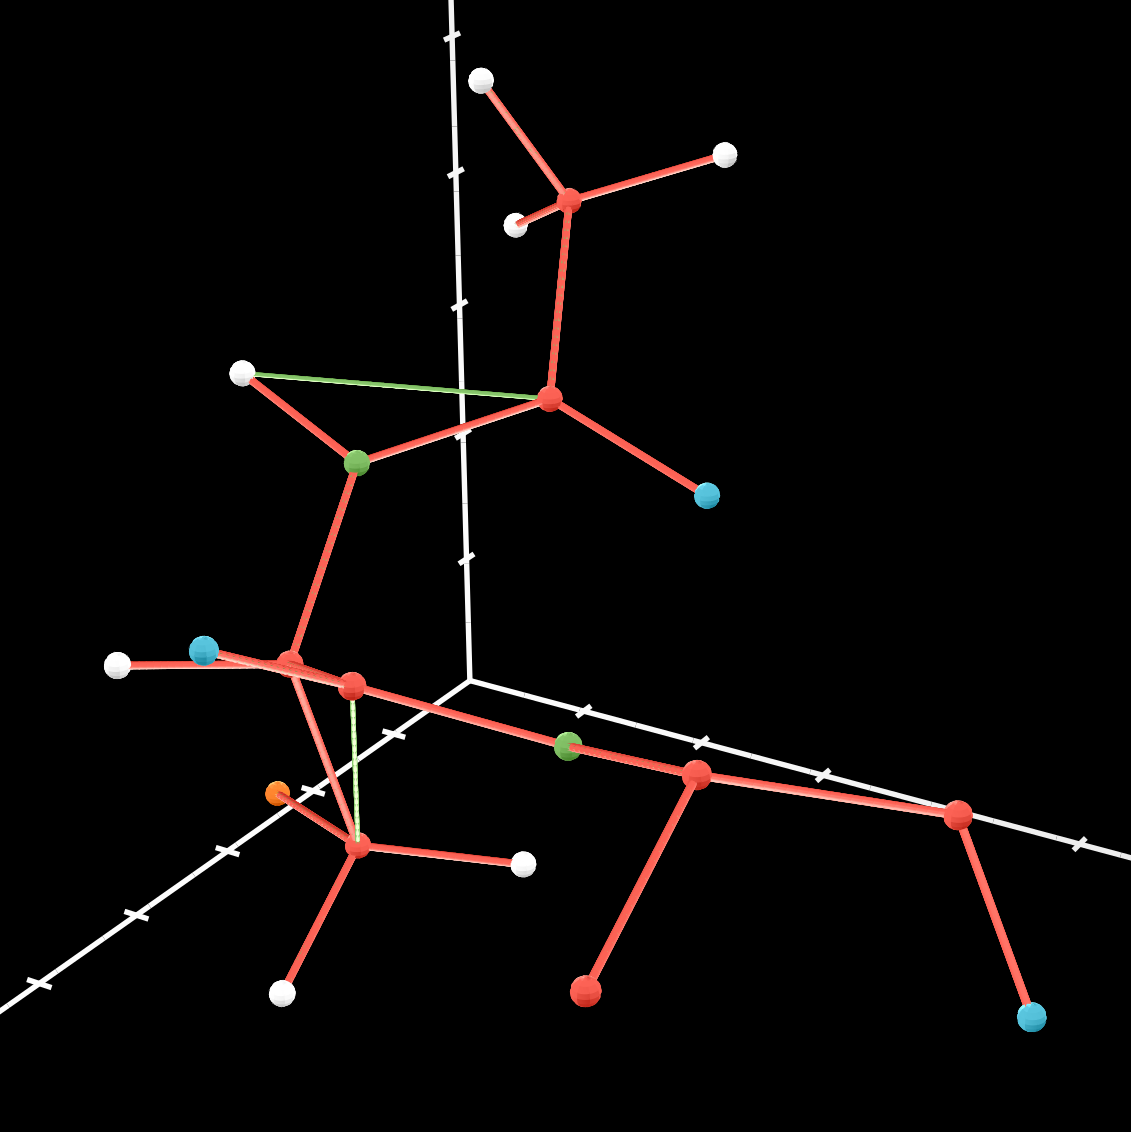
\includegraphics[height=4cm]{subgraph_lim22_1}
        \end{figure}
        \begin{figure}[!htb]
            \centering
            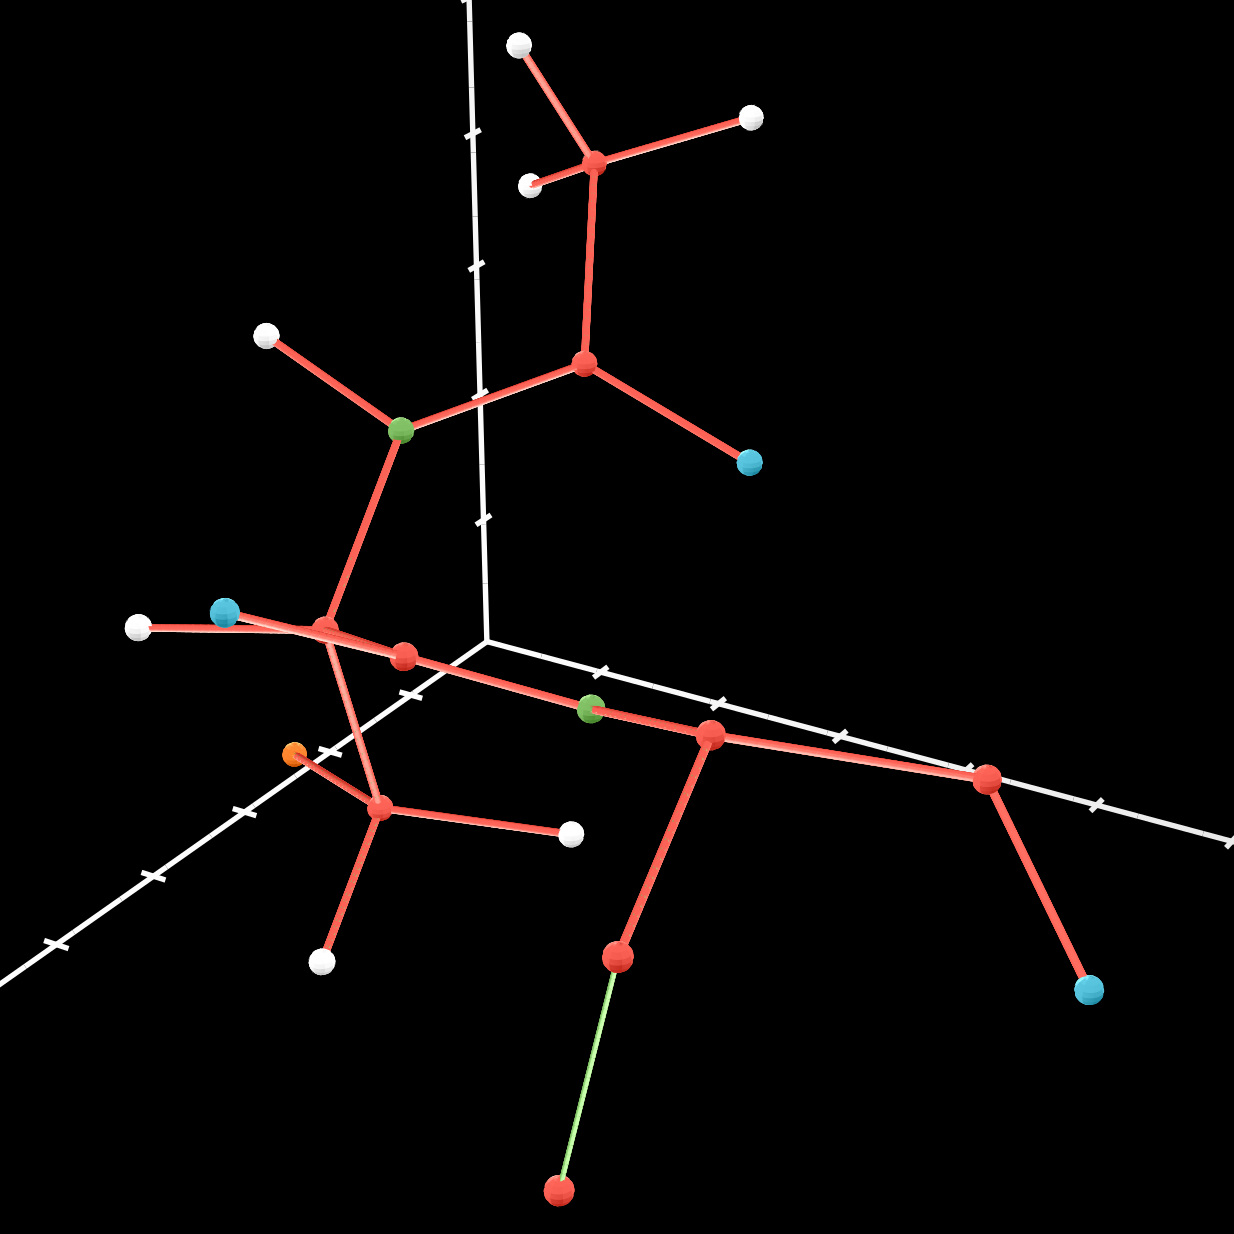
\includegraphics[height=4cm]{subgraph_lim22_2}
        \end{figure}
    \end{multicols}
    \begin{figure}
        \centering
        \caption{\label{fig:max_isom}Un sous-graphe isomorphe de taille maximale}
    \end{figure} 
    temps d'éxecution sur ce modèle : 3-4 minutes
    \begin{center}
        Cas d'égalité, sous-graphes de même taille ?
    \end{center}
\end{frame}

\subsection{Position}
\begin{frame}{Position de la sous-structure}
    $\bullet \quad$ \underline{Alignement des sous-structures isomorphes} :
    \begin{figure}[!htb]
        \centering
        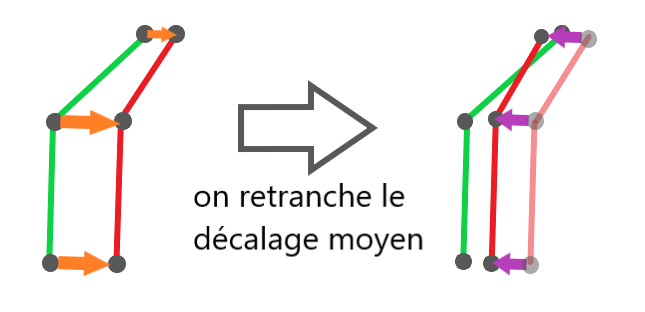
\includegraphics[width=8cm]{offset_sub}
    \end{figure}
    $\bullet \quad$ \underline{Coefficient de proximité} : \newline \newline
    branche $\quad \rightarrow \quad$ suite d'arêtes ordonnées \newline
    Même coefficient que pour les branches
\end{frame}

\subsection{Comparaison}
\begin{frame}{Comparaison de protéines}
    Une fois la plus grande sous-structure isomorphe déterminée : 
    \begin{figure}[!htb]
        \centering
        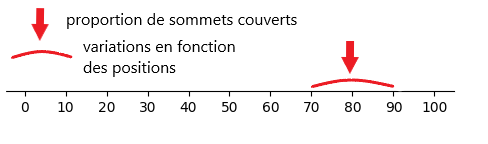
\includegraphics[width=8cm]{0to100}
        \caption{\label{fig:0to100} coefficient de proximité des protéines}
    \end{figure}
\end{frame}

\begin{frame}{Comparaison de protéines}
    \begin{multicols}{2}
        \begin{figure}[!htb]
            \centering
            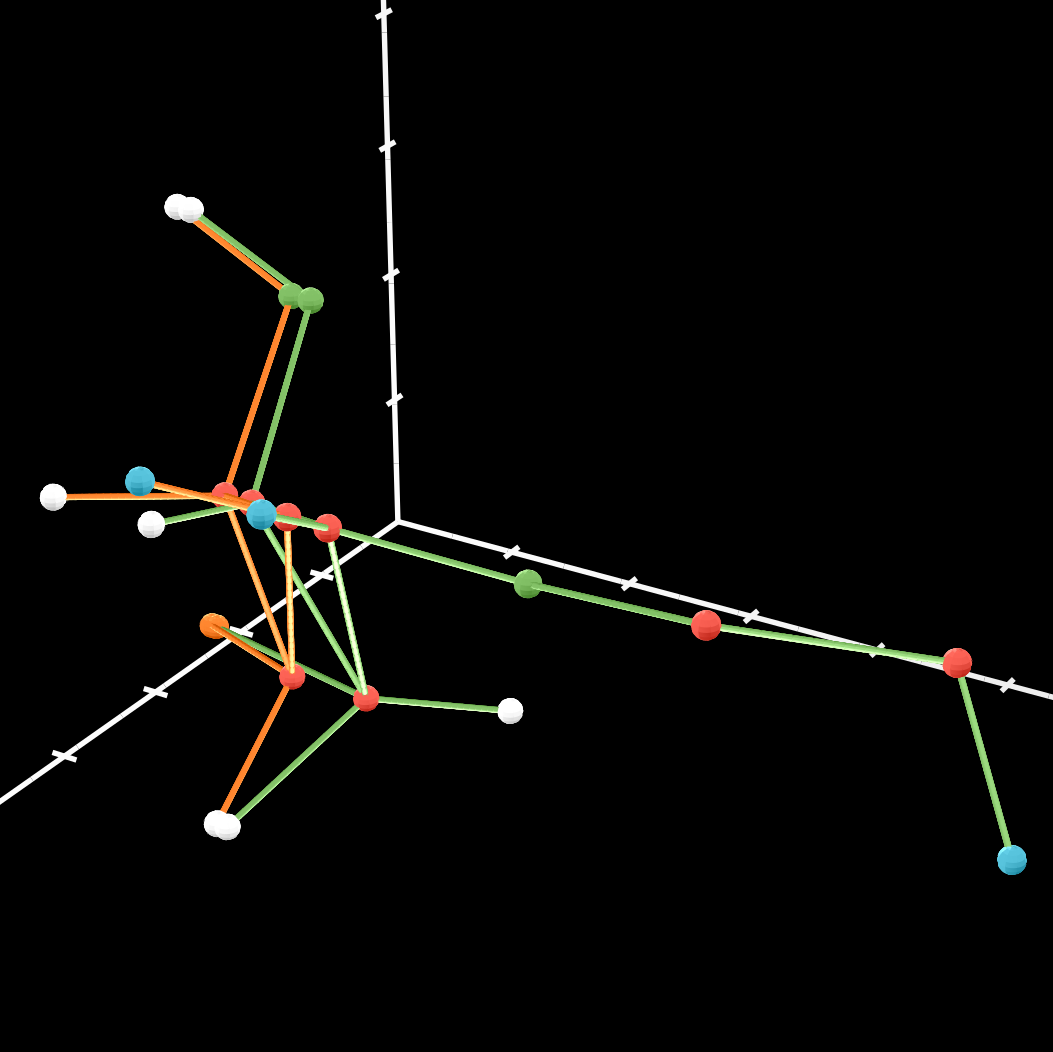
\includegraphics[width = 4cm]{comp_sub_loin}
            \caption{\label{fig: subcomp_loin} Protéines plutôt éloignées}
        \end{figure}
        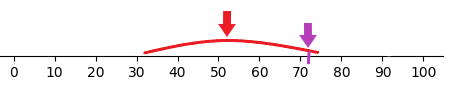
\includegraphics[width = 4cm]{0to100_loin}
        \begin{center}
            $C_{prox}=92.9 \quad C_{struct}=52$\newline \newline
            $\boxed{C=72}$
        \end{center}
    \end{multicols}
    \begin{multicols}{2}
        \begin{figure}[!htb]
            \centering
            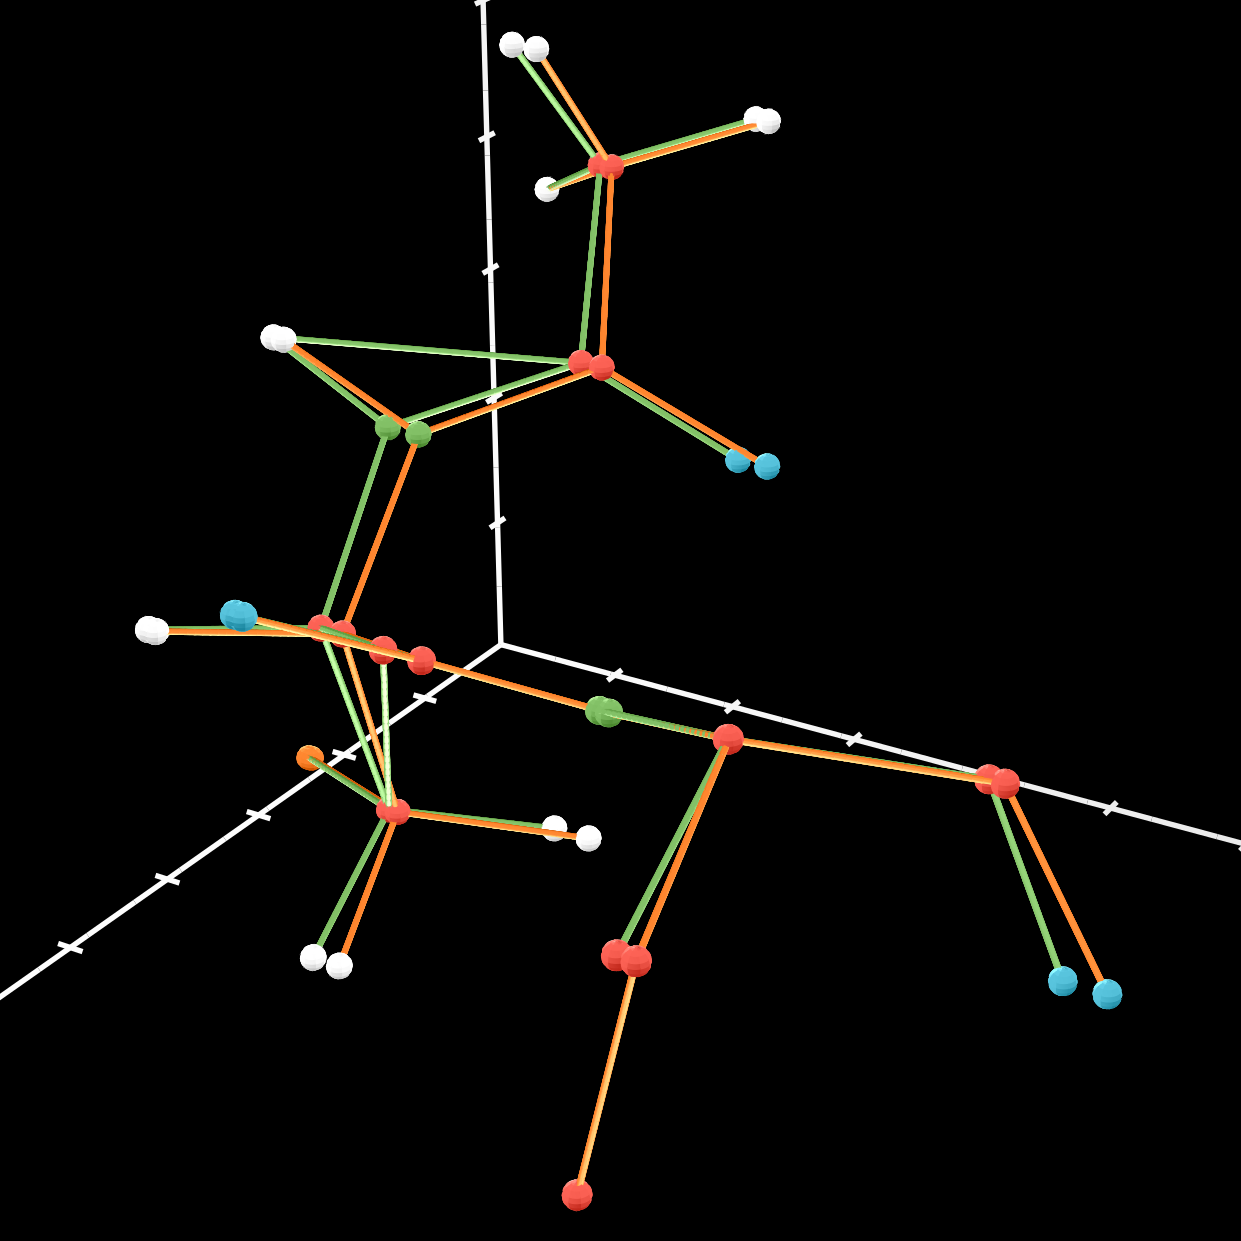
\includegraphics[width = 4cm]{comp_sub_proche}
            \caption{\label{fig: subcom_proche} Protéines plutôt proches}
        \end{figure}
        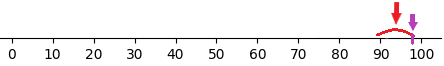
\includegraphics[width=4cm]{0to100_proche}
        \begin{center}
            $C_{prox}=97.7 \quad C_{struct}=93$\newline \newline
            $\boxed{C=96.3}$
        \end{center}
    \end{multicols}
\end{frame}

